\documentclass[twocolumn,superscriptaddress,showpacs,preprintnumbers,amsmath,amssymb,prl]{revtex4}
\usepackage{graphicx}
\usepackage{dcolumn,xcolor,ulem}
\usepackage{amsmath} 
\usepackage{amssymb}
\usepackage{amsfonts}
\usepackage{bm}
\usepackage[latin1]{inputenc}
%\usepackage{mathrsfs}

\newcommand{\cor}[1]{\textcolor{red}{#1}}
\newcommand{\change}[1]{\textcolor{blue}{#1}}
\newcommand\gp{\dot\gamma}
\newcommand\gl{\gamma_{\rm loc}}
\newcommand\gpm{\dot\gamma_{\rm min}}
\newcommand\taum{\tau_{\rm min}}

\newcommand{\ti}[1]{\textbf{\color{blue}#1}} % remarques de Thibaut
\newcommand{\titi}[1]{\sout{\textbf{\color{blue}#1}}} % remarques de Thibaut


\begin{document}

%\widowpenalty=1000
%\clubpenalty=1000
%\preprint{APS/123-QED}

%\title{Stress-induced yielding of a protein gel: the rupture of a model soft solid}

 \title{Stress-induced fracture of a biopolymer gel}

\author{M.~Leocmach}
\affiliation{Universit\'e de Lyon, Laboratoire de Physique, \'Ecole Normale Sup\'erieure de Lyon, CNRS UMR 5672, 46 All\'ee d'Italie, 69364 Lyon cedex 07, France}
\author{C.~Perge}
\affiliation{Universit\'e de Lyon, Laboratoire de Physique, \'Ecole Normale Sup\'erieure de Lyon, CNRS UMR 5672, 46 All\'ee d'Italie, 69364 Lyon cedex 07, France}
\author{N.~Taberlet}
\affiliation{Universit\'e de Lyon, Laboratoire de Physique, \'Ecole Normale Sup\'erieure de Lyon, CNRS UMR 5672, 46 All\'ee d'Italie, 69364 Lyon cedex 07, France}
\affiliation{UFR de Physique, Universit\'e Claude Bernard Lyon 1, 43 boulevard du 11 novembre, 69100 Villeurbanne, France}
\author{T.~Divoux}
\email{divoux@crpp-bordeaux.cnrs.fr}
\affiliation{Centre de Recherche Paul Pascal, CNRS UPR 8641 - 115 avenue Schweitzer, 33600 Pessac, France}
\author{S.~Manneville}
\affiliation{Universit\'e de Lyon, Laboratoire de Physique, \'Ecole Normale Sup\'erieure de Lyon, CNRS UMR 5672, 46 All\'ee d'Italie, 69364 Lyon cedex 07, France}

\date{\today}

\begin{abstract}
Biopolymer gels are known to behave qualitatively as soft solids: under external stress they display macroscopic fractures followed by an \textit{irreversible} yielding which has not been much investigated. As such, biopolymers strongly differ from the far more studied yield stress fluids such as emulsions, colloidal gels and glasses, etc. which also display a solid behavior at rest, but can be shear rejuvenated after yielding.
In this letter, combining optical and ultrasonic imaging to rheology we shed new light on the failure scenario of an acid-induced protein gel. Stress-controlled experiments reveal a brittle-like rupture: after a power-law primary creep regime, fully accounted for by the linear elastic properties of the gel, fractures nucleate and slowly grow as the log of time perpendicularly to the shear, up to the suddden rupture. The total duration of this failure process surprisingly follows a decreasing power-law with the applied shear stress, strongly reminiscent of Basquin's law of solids. These results are discussed in the frame of theoretical approaches including Fiber's Bundles Models.

%Acid-induced protein gels are soft materials that are known to behave qualitatively as soft solids. Indeed, under external shear their non-linear behavior feature macroscopic fractures followed by an \textit{irreversible} yielding, and once broken, no shear or rest period allow them to recover their initial elastic properties contrarily to soft glassy materials such as emulsions, colloidal gels and glasses, etc. which can be shear rejuvenated.

%The failure time follows a decreasing power-law with the applied shear stress strongly reminiscent of Basquin's law. 
%Our results are discussed within the frame of Fiber's Bundles Models which account for the fracture growth but fail to reproduce the scaling of the faillure time.   


%Under external stress, their non-linear behavior display brittle-like features through the growth of fractures followed by an irreversible yielding. In this letter, we report on the stress induced rupture scenario of such protein gels combining optics and ultrasonic velocimetry to rheology. We show that protein gels experience a three step rupture . The rupture time decreases as an exponentially with the applied shear-stress 
\end{abstract}

\pacs{}
\maketitle


%Under a constant external load, a solid deforms and may eventually fail. The resulting slow deformation refered as creep has been investigated over a century \cite{Andrade:1910} and differs depending on the nature of the material. Brittle materials such as ceramics, cold metals, etc. exhibit low plastic deformation prior rupture that is characterized by fast crack propagation perpendicular to the applied stress and a clear-cut fracture, whereas ductile materials such as metals at room temperature, polymers, etc. display large plastic deformation and even flow prior any rupture is observed [XXX]. Interestingly, these two categories defined for hard materials hold true for very soft solids such as viscoelastic fluids and yield stress fluids. On the one hand, ductile-like behavior is commonly observed for soft glassy materials such as emulsions, foams microgels, colloidal glass and gels, etc \cite{Gibaud:2010,Schall:2010,Divoux:2011,Siebenburger:2012,Sprakel:2011} which experience extensive plastic deformations and flow without fracture under external stress. On the other hand, brittleness has been reported on viscoelastic materials, mostly on transient networks \cite{Ligoure:2013}, and thermoreversible gels \cite{Bonn:1998,Baumberger:2006,Daniels:2007,Brenner:2013}. 


Under a constant external load, a solid deforms and may eventually fail. The resulting slow deformation refered to as {\it creep} has been investigated over a century on solid materials \cite{Andrade:1910,Nechad:2005,Miguel:2002} but only a handful of papers have dealt with such issue on soft solids \cite{Higgs:1990,vanVliet:1995}, none of which reporting local measurements. Soft solids denotes gels made through the reversible association of biopolymers such as proteins or polysaccharides and play key role in food science, from set-style yogourt or cheese, to jelly based deserts, etc. \cite{Mezzenga:2005}.
These materials behave as elastic solids under small deformations, but display remarkable non-linear behavior featuring fractures followed by irreversible rupture \cite{Bonn:1998,Baumberger:2006,Daniels:2007,Brenner:2013}. The irreversibility stems directly  from the existence of an external control parameter - the temperature (resp. the pH) in the case of thermoreversible gels (resp. acid-induced gels) - which, makes the system impossible to shear-rejuvenate after failure, contrarily to other soft glassy materials such as emulsions, colloidal gels and glasses \cite{Cloitre:2000}.

  If a great deal of effort has been made to use proteins and polysaccharides separately or mixed to design soft materials with specific mechanical properties and texture \cite{Dickinson:2006,Gibaud:2012}, their non-linear mechanical behavior under stress has been only partially addressed \cite{vanVliet:1995}. Several simple questions remain unanswered: {\it What is the spatially resolved scenario of creep and fracture under applied shear stress}? And {\it how far does the analogy with the failure scenario of brittle solid goes}? 
%%%%%%%%%%%%
\begin{figure}
\centering
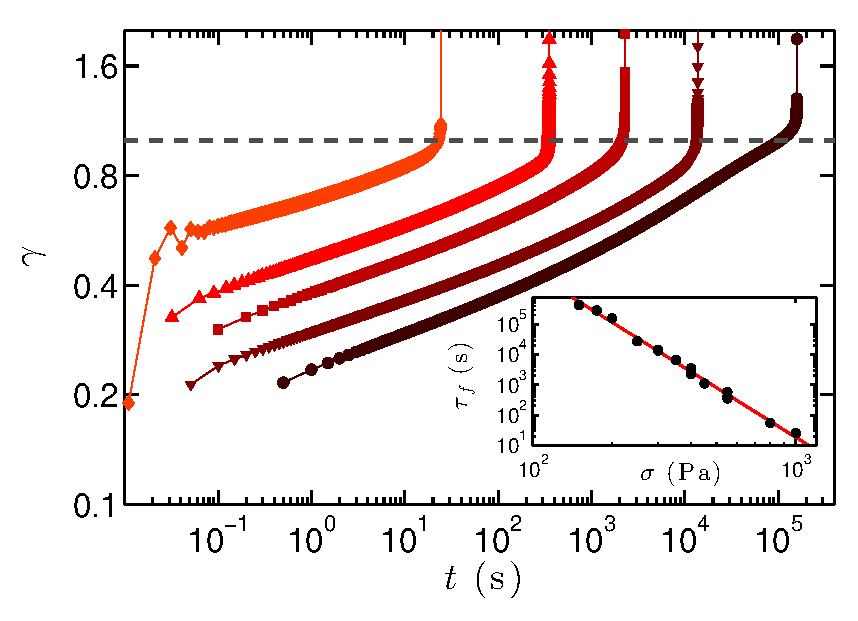
\includegraphics[width=0.9\columnwidth]{Fig1.eps}
\caption{(color online) Strain response $\gamma(t)$ in a 4\%~wt. casein gel acidified with 1\%~wt. GDL for an imposed shear stress $\sigma=200$ ($\bullet$), 300 ($\blacktriangledown$), 400 ($\blacksquare$), 550 ($\blacktriangle$), and 1000~Pa ($\blacklozenge$) from right to left. The gap width is 1~mm. The gray dotted line shows $\gamma=1$. Inset: failure time $\tau_f$ vs $\sigma$. The red line is the best power-law fit $\tau_f=A\sigma^{-\beta}$ with $\beta=5.45\pm 0.05$ and $A=40.6\pm 0.5$~s.Pa$^\beta$.
\label{fig1}}
\end{figure} 
%%%%%%%%%%%%
In the present letter, we report on the stress-induced fracture scenario of acid-induced protein gels by means of rheology coupled to optical and ultrasonic imaging. These gels are formed reversibly by acidification of sodium caseinate solution \cite{Lucey:1998}, and at fixed low pH values, display irreversible fractures under large strain \cite{vanVliet:1995} which makes them perfect candidates to quantify brittleness in biopolymer gels and tackle the above-mentioned questions. 
Here we demonstrate thanks to local measurements that under external load, these model soft solids display a brittle-like irreversible yielding which separates into three phases: $(i)$ a primary or Andrade-like creep regime during which the strain field is homogeneous in bulk, $(ii)$ a secondary creep during which fractures nucleate and grow logarithmically from the boundaries toward the center of the experimental cell and $(iii)$ a finite time singularity concomittent to the sudden failure of the gel. The failure time displays a non-trivial power-law scaling with the applied shear-stress that contrasts with the exponential scalings usually reported for solid brittle materials \cite{Vanel:2009}.


%%%%%%%%%%%%
\begin{figure}
\centering
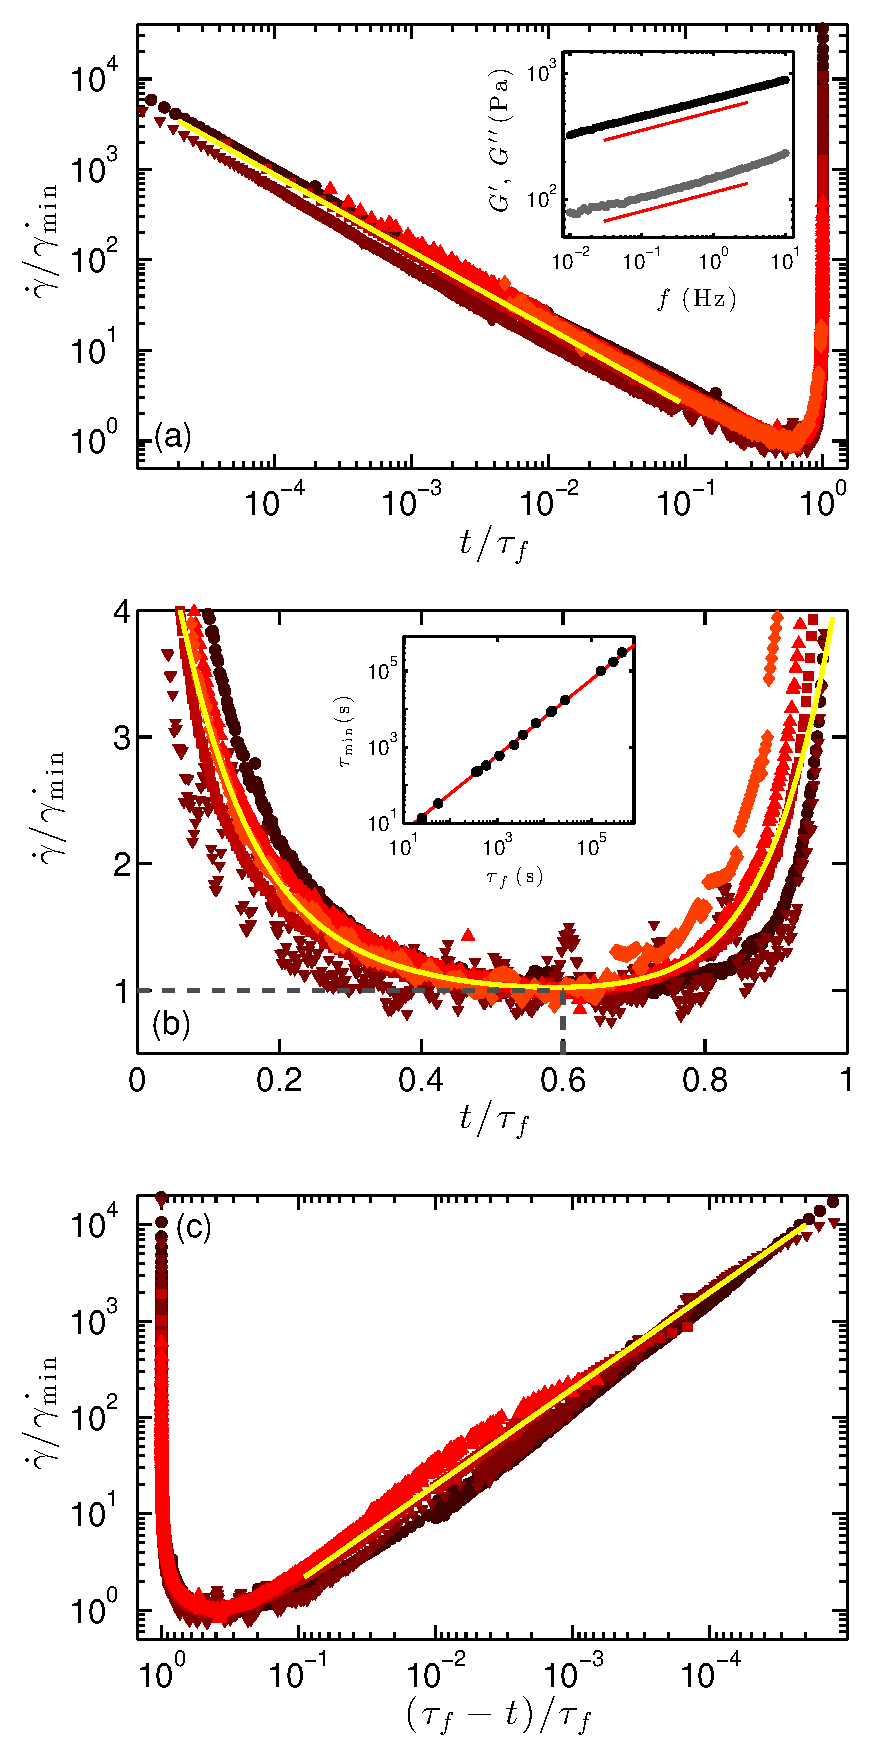
\includegraphics[width=7cm,clip]{Fig2.eps}
\caption{(color online) Normalized shear rate responses $\gp(t)/\gpm$ corresponding to the data of Fig.~\ref{fig1} and plotted so as to emphasize each of the three successive creep regimes. $\gpm$ is the minimum shear rate reached at $\taum$ (see text and Suppl. Fig.~2). (a)~Primary creep: $\gp(t)/\gpm$ vs $t/\tau_f$ in logarithmic scales. The yellow line is $\gp(t)\sim t^{-0.85}$. Inset: Linear viscoelastic moduli $G'$ (top) and $G''$ (bottom) as a function of frequency $f$ for a strain amplitude of 1XXX~\%. Red lines are power laws $G'\sim G''\sim f^{0.15}$. (b)~Secondary creep: $\gp(t)/\gpm$ vs $t/\tau_f$ in linear scales. The yellow curve is a sixth order polynomial fit to the data showing that $\taum\simeq 0.6~\tau_f$. Inset: $\taum$ vs $\tau_f$. The red line is the best linear fit $\taum=0.598\tau_f$. (c)~Tertiary creep: $\gp(t)/\gpm$ vs $(\tau_f-t)/\tau_f$ in logarithmic scales with a reversed horizontal axis. The yellow line is $\gp(t)\sim (\tau_f-t)^{-1}$. 
\label{fig2}}
\end{figure} 
%%%%%%%%%%%%

\textit{Experimental set-up and protocol.-} Gels are prepared by disolving 4\% wt. of sodium caseinate powder (Firmenich) in demineralized water under gentle mixing (XX rpm) at T$=35^{\circ}$C. To induce the gelation, the solution is acidified with 1\% wt. glucono-$\delta$-lactone (GDL) in powder (Firmenich). The solution is then stirred for the GDL to dissolve before being poured into the gap of a polished Plexiglas Couette cell (height 50~mm, inner rotating cylinder 23~mm, outer fixed cylinder 25~mm, gap e=2~mm) immersed into a temperature controlled water tank at T=(25.0$\pm$0.1)$^{\circ}$C. Rheological data are recorded during the gel formation  via a stress-controled rheometer (ARG2, TA Instruments) through small amplitude oscillatory shear (see Fig.~1 in the Supplemental Material). The gelation is over when the increasing linear elastic ($G'$) and viscous ($G''$) modulii reach a plateau with $G'>G''$. A constant stress is then applied to the sample. Images of the gel are recorded simultaneously to the rheology thanks to a webcam (XXX). Displacement field and velocity maps in the (r, z) plane can also be recorded simultaneously to rheology by a custom-made ultrasonic scannner detailed in \cite{Gallot:2013}. In this case, the solution is seeded prior to the acidification with accoustic tracers -here 3\% wt. polyamide spheres, of diameter 10~$\mu$m (Orgasol 2002 EXD Nat 1, Arkema) that do not modify the final gel properties [see Supplemental Fig.~\ref{suppfig1}~(b)]. Yielding being irreversible, each creep experiment requires to prepare a new sample in-situ.  

%%%%%%%%%%%%
\begin{figure*}[t]
\centering
\includegraphics[width=18cm,clip]{Fig3.eps}
\caption{(color online) Ultrasonic images (left) and direct visualization of the Couette cell (right) recorded simultaneously at various times in the primary [(a)~$t/\tau_f=0.02$], secondary [(b)~$t/\tau_f=0.57\simeq\taum/\tau_f$], and tertiary  [(c) $t/\tau_f=0.93$ and (d) 0.99] creep regimes. Ultrasonic images are velocity maps $v(r,z,t)$ computed by averaging over 4~s and coded using the linear color levels shown below the images, whose position relative to the picture of the cell reflects the actual arrangement of the ultrasonic probe along the vertical direction $z$. Experiment performed on a 4\%~wt. casein gel seeded with 3\%~wt. polyamide spheres and acidified with 1\%~wt. GDL under $\sigma=300$~Pa. The gap width is 2~mm. See also Suppl. Movie~1.
\label{fig3}}
\end{figure*} 
%%%%%%%%%%%%


\textit{Macroscopic behaviour.-} Under constant applied shear stress $\sigma$, the global deformation $\gamma$ displays the same robust evolution with time (Fig.~\ref{fig1}): it grows almost logarithmicaly with time up to $\gamma \sim 1$, than accelerates up to the moment the gel breaks. 
 The failure time $\tau_f$ of the gel decreases as a power-law of $\sigma$ [Fig.~\ref{fig1}~(inset)] and allow us to rescal all the experiments on a single mastercurve.[see fig.~\ref{suppfig2} in the Supplemental Materials]
Figure~\ref{fig2} displays such mastercurve as the temporal evolution of the shear rate $\dot \gamma$ and each subplot (a), (b) and (c) uses a scale that lay the emphasis respectively on the primary, the secondary and the tertiary regime.
In the primary creep regime [Fig.~\ref{fig2}~(a)], shear rates decrease as the following power-law:  $\dot \gamma(t) \sim~\dot \gamma_{min} (t/\tau_f)^{-\alpha}$, with $\alpha=0.85$ recalling the primary creep observed in solids refered to as the Andrade creep \cite{Miguel:2002}. Interestingly, here this scaling is directly linked to the linear viscoelasticity which predicts for such power-law creep the following scaling: $G(\omega) \sim \omega^{1-\alpha}$. Inset of figure~\ref{fig2}~(a) confirms that $G'(\omega)$ and $G"\sim \omega ^{0.15}$, strongly suggesting that the primary creep is purely elastic.
During the secondary creep regime, the shear-rate reaches a minimum value at $t=\tau_{min}= (0.61\pm0.04)\tau_f$ independently of the applied stress [Fig.~\ref{fig2}~(b)-(inset)] as similarly reported for solid composite materials \cite{Nechad:2005}, colloidal gels of attractive particles \cite{Grenard:2013} and Fiber Bundles Models \cite{Kovacs:2008,Jagla:2011}. 
In the tertiary creep regime, the shear rate increases by several orders of magnitude scaling as $(\tau_f-t)^{-1}$ and display a finite time singularity. Finally, the failure time of the gel is a decreasing function of the applied shear stress in agreement with what has been reported qualitativeley in similar systems \cite{vanVliet:1995}, and scales as the following power-law: $\tau_f \sim \sigma^{-5.45\pm 0.05}$, a key result on which we come back in the discussion section.

\textit{Local behaviour.-} Local measurements allow us to get deeper insight into the creep regimes [see movie~1 in the Supplemental material]. During the primary regime, no cracks or failure can be seen from direct visualization [Fig.~\ref{fig3}.~(a)] while ultrasonic imaging reveals that within the spatial resolution of a few microns, the strain field is homogeneous [Fig~\ref{fig4}~(b)]. If plastic events take place in this primary regime, they occur at smaller scale. However, given the agreement between the Andrade exponent and the frequency scaling of the linear elastic modulus discussed above, it is more likely that no or a negligible amount of plastic events take place during this regime, coroborating the optical and ultrasonic measurements. 
In the secondary creep, fractures nucleate from the top and bottom edges of the Couette cell and start growing perpendicularly to the shear. In agreement, velocity maps become heterogeneous [Fig.~\ref{fig3}.~(b)-(c)] and display intermittent fluctuations along the cell height corresponding to the independant growth of the vertical cracks [Fig~\ref{fig4}~(d)]. 
In the tertiary creep regime, cracks have grown along the vorticity, in a periodic fashion in the orthoradial direction while the velocity map directly correlates with the crack growth [Fig.~\ref{fig3}.~(d)]. Finally, over secondary and tertiary regimes, direct visualization and ultrasonic velocimetry show that the cracks display a continuous logarithmic growth with no remarkable change between the two regimes [Fig~\ref{fig4}~(e)].
Note that these three regimes do not depend on the geometry, and are also observed to be quantitatively the same in plate-plate geometry [see movie~2 in the Supplemental Materials].

\textit{Discussion.-} As a central result, acid-induced casein gels display a remarkable brittle-like rupture scenario, different from other soft materials such as transient-network systems \cite{Ligoure:2013}, because truly irreversible. The pH is key to the irreversibility and plays the role of an additional control parameter that, when maintained at values lower than the isoelectric point, prevent the system from healing.
Comparatively, Yield Stress Fluids (YSF) that display a solid-like behavior at rest, either because of a jammed microstructure or attractive interactions \cite{Sciortino:2005,Bonnecaze:2010}, but do not present such external control parameter, display a similar rheological signature during their stress-induced yielding. Indeed the S-shaped curved pictured in figure~\ref{fig2}~(a) has been also reported in \cite{Bauer:2006,Gibaud:2010,Divoux:2011,Siebenburger:2012,Grenard:2013}. However, their yielding scenario is fundamentally different. Local measurements conducted on both type of soft glassy materials have revealed that no fractures take place in the bulk: the microstructure rather reorganizes and flows in a ductile way. Our study reveals that acid-induced gels behave elastically up to the rupture point and that fractures develop and grow logarithmically, perpendicularly to the shear direction prior an irreversible failure which makes casein gels model {\it brittle soft solids}.

%%%%%%%%%%%%
\begin{figure*}
\centering
\includegraphics[width=18cm,clip]{Fig4.eps}
\caption{(color online) (a)~Local velocity $\langle v(r,z,t)\rangle_z$ and (b)~local strain field $\langle\gl(r,z,t)\rangle_z$ averaged over the vertical direction $z$ at various times during primary creep: $t/\tau_f=1.9\,10^{-3}$ (black $\bullet$), $1.7\,10^{-2}$ (blue $\blacktriangledown$), and 0.15 (red $\blacksquare$). Solid lines are linear profiles. (c)~Spatiotemporal diagram of the local velocity $\langle v(r,z,t)\rangle_r$ averaged over the radial direction $r$ and plotted in linear color levels as a function of $z$ and $t/\tau_f$. (d)~Standard deviation $\delta_z v(t)$ of $\langle v(r,z,t)\rangle_r$ taken over the vertical direction $z$ (thick black line) together with corresponding standard deviation $\delta_r v(t)$ computed over the radial direction $r$ on the $z$-average $\langle v(r,z,t)\rangle_z$ (thin red line). (e)~Fracture length $\ell(t)$ vs $(\tau_f-t)/\tau_f$ as inferred from direct visualization ($\bullet$, average over 6 different fractures, error bars show the standard deviation) and from ultrasonic imaging ($\circ$) and normalized by the height $H$ of the Couette cell. Gray dots show the visualization data for the longest fracture which leads to the failure of the sample at $\tau_f$. Red lines are the best fits $\ell(t)=\alpha+\beta\log(1-t/\tau_f)$ to the visualization data. Same experiment as in Fig.~\ref{fig3}. See also Suppl. Movie~1.
\label{fig4}}
\end{figure*} 
%%%%%%%%%%%%

Let us examine in more detail the rupture process and compare it to what is seen on brittle solid materials. Here, the primary creep and its power-law exponent ($\dot \gamma \sim t^{-\alpha}$, with $\alpha=0.85$) is fully accounted for by the linear rheology while local measurements reveals in agreement an homogeneous bulk deformation. This result strongly contrasts with the primary creep of both solid materials and YSFs \cite{Bauer:2006,Divoux:2011,Siebenburger:2012,Grenard:2013} that usually exhibit a power-law creep with slightly smaller exponents (0.3 $\leq \alpha \leq 0.7$) that are not directly related to linear rheology. Besides, the linear behavior of YSF generally differs from a simple power-law scaling, while in the case of solids, the primary creep is irreversible and has been attributed to dislocation interactions in the case or cristaline materials \cite{Miguel:2002} or localized plastic rearragements which nature is still unclear in amorphous materials \cite{Rosti:2010}. \ti{ XXX The exponent in the case of casein gel is robust and neither depend on the geometry nor on the GDL concentration within the explored range ... mentioned or left aside for the long paper? XXX}

The second key feature of the failure process of casein gels is the logarithmic growth of fractures observed in the second and tertiary creep regimes [Fig.~\ref{fig4}~(d)]. Such evolution  has been also reported on solid disordered materials displaying brittle rupture (such as paper) and interpreted in the framework of Griffith-like or Local Energy Barrier (LEB) models \cite{Vanel:2009}. However, these approaches predict an exponential scaling of the rupture time with the applied stress, which gives a less convincing fit of the experimental data than the decreasing power-law we proposed in figure~\ref{fig1}~(inset). This result strongly suggests that another mechanism is at stake in the failure process of casein gels.
\ti{XXX 1) Should we discuss in more details the LEB and Griffith models? 2) Should we mention that the log growth differs from the algebric growth of capillary fractures observed in thermo-reversible gels \cite{Daniels:2007} ?? XXX}

The last key feature of this brittle scenario is the power-law dependance of the failure time with the applied shear stress...XXX

\begin{itemize}
\item FBM are relevant here because the gel microstructure is formed of strands \cite{Kalab:1983,Roefs:1990}. FBM that rely on elastic fibers with a local yield strain (or stress) and introduce a non-linear Eyring rheology or a local coupling lead to a different scaling law than the one we find here for the failure time with the applied stress. In their law appears a ``yield stress" \cite{Kun:2003,Nechad:2005,Kovacs:2008,Jagla:2011} that is not present here. The promising approach combines elastic fibers with a local yield strain and take into account damage accumulation as in \cite{Kun:2007,Halasz:2012}. 
\item Idem Compare to the scalings observed in YSF - in particular microgels display a similar power-law scaling, except that the yield point appears explicitely in the scaling as the critical point in a dynamical phase transition \cite{Divoux:2012}. Propose an explenation or at least raise a point.
\item re-Read \& mention somewhere the following ref. \cite{Chaudhuri:2013} 
\item Note for us, that some materials display a brittle or a ductile behavior depending on the strain-rate they experience - see the review by Mikko Alava on ``paper" or even foams- travail de J.C Tsai. It urges for systematic step shear experiments on casein gels :-).
\item conclude   
\end{itemize}




%Acidification is reversible: one can switch reversibly from the gel to the casein solution by tuning the pH respectively below or the casein isoelectric point (pH$\sim$~4.6).    


\begin{acknowledgments}
The authors thank Thomas Gibaud for fruitful discussions, Miloslav Kal\'ab for kindly providing us with unobtainable references and Alan Parker for precious advice and for providing the casein and GDL. This work was funded by the Institut Universitaire de France and by the European Research Council under the European Union's Seventh Framework Programme (FP7/2007-2013) / ERC grant agreement No.~258803. 
\end{acknowledgments}

\begin{thebibliography}{}

\bibitem{Andrade:1910} E.N. Da C. Andrade Proc. R. Soc. London A {\bf 84}, 1 (1910).

\bibitem{Nechad:2005} H. Nechad et al., Phys. Rev. Lett. {\bf 94}, 045501 (2005); J. Mech. Phys. Solids {\bf 53}, 1099-1127 (2005).

\bibitem{Miguel:2002} M.C. Miguel, A. Vespignani, M. Zaiser and S. Zapperi, Phys. Rev. Lett. {\bf 89}, 165501 (2002); M.C. Miguel, L. Laurson and M.J. Alava, Eur. Phys. J. B {\bf 64}, 443--450 (2008).

\bibitem{Higgs:1990} P.G. Higgs and S.B. Ross-Murphy, Int. J. Biol. Macromol. {\bf 12}, 233--240, (1990).

\bibitem{vanVliet:1995} T. van Vliet and P. Walstra, Faraday Discuss. {\bf 101}, 359--370 (1995); T. van Vliet, H.J.M. van Dijk, P. Zon and P. Walstra, Colloid Polym. Sci. {\bf 269}, 620--627 (1991); L.G.B. Bremer et al., Colloids Surf. {\bf 51}, 159--170 (1990).

\bibitem{Mezzenga:2005} R. Mezzenga, P. Schurtenberger, A. Burbidge and M. Michel, Nature Materials {4}, 729--740 (2005).

\bibitem{Brenner:2013} T. Brenner et al., J. Non-Newtonian fluid Mech. {\bf 196}, 1--7 (2013).

\bibitem{Bonn:1998} D. Bonn et al., Science {280} 265--267 (1998).

\bibitem{Baumberger:2006} T. Baumberger, C. Caroli and D. Martina, Nature Materials {\bf 5}, 552-555 (2006).

\bibitem{Daniels:2007} K. Daniels et al., Phys. Rev. Lett. {\bf 99}, 124501 (2007).

\bibitem{Cloitre:2000} M. Cloitre, R. Borrega and L. Leibler, Phys. Rev. Lett. {\bf 85} 4819--4822 (2000); V. Viasnoff and F. Lequeux, Phys. Rev. Lett. {\bf 89} 065701 (2002); Coussot et al., Phys. Rev. Lett. {\bf 88}, 175501 (2002).

\bibitem{Dickinson:2006} E. Dickinson, Soft Matter {\bf 2}, 642--652 (2006).

\bibitem{Gibaud:2012} T. Gibaud et al., Faraday Discuss., {\bf 158}, 267--284 (2012).

\bibitem{Lucey:1998} J.A. Lucey and H. Singh, Food Research Int. {\bf 30}, 529--542 (1998).

%\bibitem{vanVliet:1991} T. van Vliet, H.J.M. van Dijk, P. Zon and P. Walstra, Colloid Polym. Sci. {\bf 269}, 620--627 (1991).

%\bibitem{Bremer:1990} L.G.B. Bremer et al., Colloids Surf. {\bf 51}, 159--170 (1990).

\bibitem{Vanel:2009} L. Vanel et al., J. Phys. D: Appl. Phys. {\bf 42} 214007 (2009).

\bibitem{Gallot:2013} T. Gallot et al., Rev. Sci. Instrum. {\bf 84}, 045107 (2013).

\bibitem{Grenard:2013} V. Grenard, T. Divoux, N. Taberlet and S. Manneville, Soft Matter (2013) - DOI: 10.1039/C3SM52548A 

\bibitem{Jagla:2011} E.A. Jagla, Phys. Rev. E {\bf 83} 046119 (2011).

\bibitem{Kovacs:2008} K. Kov\'acs et al., Phys. Rev. E \textbf{77}, 036102 (2008).

\bibitem{Sciortino:2005} F. Sciortino and P. Tartaglia, Advances in Physics {\bf 54}, 471--524 (2005).

\bibitem{Bonnecaze:2010} R.T. Bonnecaze and M. Cloitre, Adv. Polym. Sci. {\bf 236}, 117--161 (2010).

\bibitem{Bauer:2006} T. Bauer, J. Oberdisse and L. Ramos, Phys. Rev. Lett. {\bf 97}, 258303 (2006).

\bibitem{Divoux:2011} T. Divoux, C. Barentin and S. Manneville, Soft Matter {\bf 7}, 8409--8418 (2011).

\bibitem{Siebenburger:2012} Siebenb\"urger, M. Ballauff and T. Voigtmann, Phys. Rev.
Lett., {\bf 108}, 255701 (2012)

\bibitem{Gibaud:2010} T. Gibaud, D. Frelat and S. Manneville, Soft Matter {\bf 6}, 3482--3488 (2010).

\bibitem{Rosti:2010} J. Rosti, J. Koivisto, L. Laurson, M.J. Alava, Phys. Rev. Lett. {\bf 105}, 100601 (2010).

%\bibitem{Sprakel:2011} J. Sprakel et al., Phys. Rev. Lett. {\bf 106}, 248303 (2011).

\bibitem{Kun:2003} F. Kun et al., Phys. Rev. E {\bf 67} 061802 (2003).

%\bibitem{Ghofraniha:2012} N. Ghofraniha et al., Soft Matter {\bf 8}, 6214 (2012).

\bibitem{Ligoure:2013} C. Ligoure and S. Mora, Rheol. Acta {\bf 52}, 91-114 (2013).

\bibitem{Kun:2007} F. Kun et al., J. Stat. Mech. P02003 (2007); F. Kun et al., Phys. Rev. Lett. {\bf 100}, 094301 (2008).

\bibitem{Roefs:1990} S.P.F.M. Roefs, A.E.A. De Groot-Mostert and T. Van Vliet, Colloids Surf. {\bf 50}, 141--159 (1990).

\bibitem{Kalab:1983} M. Kal\'ab, P. Allan-Wojtas and B.E. Phipps-Todd, Food Microstructure {\bf 2}, 51--66 (1983).

\bibitem{Divoux:2012} T. Divoux, D. Tamarii, C. Barentin, S. Teitel and S. Manneville, Soft Matter {\bf 8}, 4151---164 (2012).

\bibitem{Halasz:2012} Z. Hal\'asz, Z. Danku and F. Kun, Phys. Rev. E {\bf 85}, 016116 (2012).

%\bibitem{Roefs:1986} S.P.F.M. Roefs, {\it Structure of acid casein gels. A study of gels formed after acidification in the cold. PhD Thesis}, Wageningen Agricultural University, The Netherlands (1986).

%\bibitem{Schall:2010} P. Schall and M. van Hecke, Annu. Rev. Fluid Mech. {\bf 42} 67--88 (2010).

\bibitem{Chaudhuri:2013} P. Chaudhuri and J. Horbach, Phys. Rev. E {\bf 88}, 040301(R) (2013).


\end{thebibliography}


\clearpage
\newpage
\setcounter{figure}{0}

\section*{\large Supplemental material}

\subsection*{Supplemental movies}

Supplemental Movie~1 shows the creep experiment analyzed in Figs.~\ref{fig3} and \ref{fig4} and performed under $\sigma=300$~Pa on a 4\%~wt. casein gel seeded with 3\%~wt. polyamide spheres and acidified with 1\%~wt. GDL. The gap width of the Couette cell is 2~mm and its height is 60~mm. Images recorded by a standard webcam are shown on the top left. Velocity maps $v(r,z,t)$ inferred from ultrasonic imaging by averaging over 4~s are shown on the top right using linear color levels. The vertical position $z=0$ on the ultrasonic images corresponds to about 20~mm below the top of the Couette cell. The two bottom graphs show the shear rate response $\gp(t)$ (left) and the strain response $\gamma(t)$.

Supplemental Movie~2 shows the failure of a 4\%~wt. casein gel acidified with 1\%~wt. GDL in a plate-plate geometry for an imposed shear stress $\sigma=XXX$~Pa. The plate diameter is 40XXX~mm and the gap width is 1XXX~mm. In this case fractures grow parallel to the vorticitty direction, i.e. along the radial direction. The shear rate response is fully similar to that in the Couette geometry.

\subsection*{Supplemental figures} 

Figure~\ref{suppfig1} display the gelation process of a 4\%. sodium caseinate solution seeded with 3\% wt. polyamide spheres. The glucono-$\delta$-lactone contains an ester function which, once added to the solution, hydrolyzes spontaneously and leads to a slow decrease of the pH [Fig.~\ref{suppfig1}~(a)] towards the casein isoelectric point (pH$\simeq 4.6$) at which casein particles start to aggregate. The gelation starts in fact earlier at pH=5 as already discussed in \cite{Lucey:1998supp}. At this point, the elastic and viscous modulii display a brutal increase, then overshoot and converge toward their steady state values, where $G'~>~G''$. Note that the maximum of the overshoot is reached at the isoelectric point. The decrease of both modulii at lower pH is usually attributed to the overacidification which enhances the repulsive electrostatic interactions between caseinate particles of net positive charge \cite{Dickinson:2002supp}.   

 %%%%%%%%%%%%
\begin{figure}[h]
\centering
\includegraphics[width=7cm,clip]{SuppFig1.eps}
\caption{(color online) Gelation process of a 4\%~wt. casein suspension seeded with 3\%~wt. polyamide spheres and acidified with 1\%~wt. GDL. (a)~pH vs time $t$. (b)~Linear viscoelastic moduli $G'$ (top, in blue) and $G''$ (bottom, in red) recorded as a function of time $t$ for fixed frequency $f=1$~Hz and strain amplitude 0.1XXX~\%. Dashed lines indicate that the system starts to build significant elastic properties when the pH decreases below about 5. Lighter colors in (b) correspond to a sample free of polyamide spheres, showing that the addition of acoustic contrast agents does not affect significantly the gelation process and the final viscoelastic properties of the gel.
\label{suppfig1}}
\end{figure} 

 %%%%%%%%%%%%
\begin{figure}[h]
\centering
\includegraphics[width=7cm,clip]{SuppFig2.eps}
\caption{(color online) Shear rate response $\gp(t)$ in a 4\%~wt. casein gel acidified with 1\%~wt. GDL for an imposed shear stress $\sigma=200$ ($\bullet$), 300 ($\blacktriangledown$), 400 ($\blacksquare$), 550 ($\blacktriangle$), and 1000~Pa ($\blacklozenge$) from right to left. The gap width is 1~mm. The yellow line shows the power-law behavior $\gp(t)\sim t^{-0.85}$.
\label{suppfig2}}
\end{figure} 
%%%%%%%%%%%%

\begin{thebibliography}{}

\bibitem{Lucey:1998supp} J.A. Lucey and H. Singh, Food Research International A {\bf 30}, 529--542 (1998).

\bibitem{Dickinson:2002supp} E. Dickison and L.M. Merino, Food Hydrocolloids {\bf 16}, 321--331 (2002).

\end{thebibliography}

\end{document}
